\documentclass{article}
\usepackage[a4paper,
            bindingoffset=0.2in,
            left=1in,
            right=1in,
            top=1in,
            bottom=1in,
            footskip=.25in]{geometry}
\usepackage{tikz}
\usetikzlibrary{quotes,angles}

\begin{document}
\pagenumbering{gobble}
\section*{Pythagorean Theorem Proof}
\subsection*{By: Noah Chappell}

\subsection*{\underline{Theorem}:}
Given a right triangle with a hypotenuse of side length C and non-hypotenuse side lengths of A and B, $A^2+B^2=C^2$.
We can also represent the angle between sides A and C as {$\alpha$} and the angle between sides B and C as {$\beta$}.

\begin{center}
    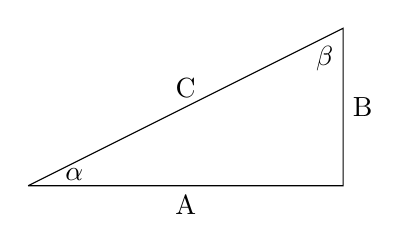
\begin{tikzpicture}
        \draw (0,0) coordinate (a) 
        -- node[below]{A}(4,0) coordinate (b) 
        -- node[right]{B}(4,2)  coordinate (c) 
        -- node[above]{C}(a)
        pic["$\alpha$", angle radius=1cm]{angle=b--a--c}
        pic["$\beta$", angle radius=0.75cm]{angle=a--c--b};
    \end{tikzpicture}
\end{center}

\subsection*{\underline{Proof}:}

Suppose we create two identical right triangles and position the two triangles in a way so that their 
A side and B side create one line, the resulting angle between {$\alpha$} and {$\beta$} being 90°. Then 
connect the triangles with a line from their unconnected {$\alpha$} and {$\beta$} corners\\
\begin{center}
    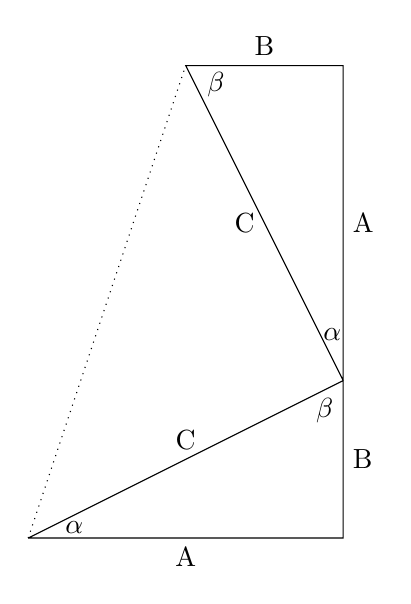
\begin{tikzpicture}
        %triangle1
        \draw (0,0) coordinate (a1) 
        -- node[below]{A}(4,0) coordinate (b1) 
        -- node[right]{B}(4,2)  coordinate (c1) 
        -- node[above]{C}(a1)
        pic["$\alpha$", angle radius=1cm]{angle=b1--a1--c1}
        pic["$\beta$", angle radius=0.75cm]{angle=a1--c1--b1};

        %triangle2
        \draw (4,2) coordinate (a2) 
        -- node[right]{A}(4,6) coordinate (b2) 
        -- node[above]{B}(2,6)  coordinate (c2) 
        -- node[left]{C}(a2)
        pic["$\alpha$", angle radius=1cm]{angle=b2--a2--c2}
        pic["$\beta$", angle radius=0.75cm]{angle=a2--c2--b2};

        %connecting line
        \draw[dotted] (a1) -- (c2);
    \end{tikzpicture}
\end{center}
We can create two equations to represent the area of this new shape:\\
The first equation sees the shape as 3 triangles while the second equation sees the shape as a trapezoid\\
\begin{center}
    $Area=2\frac{1}{2}AB+\frac{1}{2}C^2$ and $Area=\frac{1}{2}(A+B)(A+B)$
\end{center}
If we set the equations equal to each other and simplify:\\
\begin{center}
    $2\frac{1}{2}AB+\frac{1}{2}C^2=\frac{1}{2}(A+B)(A+B)$\\
    $AB+\frac{1}{2}C^2=\frac{1}{2}(A^2+2AB+B^2)$\\
    $AB+\frac{1}{2}C^2=\frac{1}{2}A^2+AB+\frac{1}{2}B^2$\\
    $\frac{1}{2}C^2=\frac{1}{2}A^2+\frac{1}{2}B^2$\\
    $C^2=A^2+B^2$\\
\end{center}
Therefore given a right triangle with a hypotenuse of side length C and non-hypotenuse side lengths of A and B, $A^2+B^2=C^2$.\\
\begin{flushright}
    
\begin{tikzpicture}
        \filldraw[fill=black](0,0) rectangle (0.3,0.3);
    \end{tikzpicture}
\end{flushright}

\end{document}
